\documentclass[12pt,reqno,a4paper]{report}
\usepackage{setspace}
\usepackage{amsmath}
\usepackage{amsfonts}
\usepackage{amssymb}
\usepackage{bbm, subfigure, appendix, graphicx}
\usepackage{tikz}
\usetikzlibrary{shapes,arrows,trees,snakes}
\usepackage[
pdftitle={dendroDoc},
pdfcreator={pdftex},
hyperindex = {true},
colorlinks = {true},
linkcolor = {blue},
citecolor = {blue}
]{hyperref} 

\usepackage{listings}
\usepackage{color}

%------------------------------------------------------------
\newtheorem{algorithm}{\textbf{Algorithm}}
\newtheorem{axiom}{Axiom}
\newtheorem{case}{Case}
\newtheorem{claim}{Claim}
\newtheorem{conclusion}{Conclusion}
\newtheorem{condition}{Condition}
\newtheorem{conjecture}{Conjecture}
\newtheorem{criterion}{Criterion}
\newtheorem{example}{Example}
\newtheorem{exercise}{Exercise}

\newtheorem{notation}{Notation}
\newtheorem{problem}{Problem}

\newtheorem{remark}{Remark}
\newtheorem{prop}{Property}
\newtheorem{define}{Definition}
\newtheorem{solution}{Solution}
\newtheorem{summary}{Summary}
\numberwithin{equation}{section}
%------------------------------------------------------------
\newcommand{\pe}{\psi}
\newcommand{\argmax}[1]{\ensuremath{\arg \,\underset{#1}{\max}\;}}
\def\d{\delta} 
\def\ds{\displaystyle} 
\def\e{{\epsilon}} 
\def\eb{\bar{\eta}}  
\def\enorm#1{\|#1\|_2} 
\def\Fp{F^\prime}  
\def\Kc{{\cal K}} 
\def\norm#1{\|#1\|} 
\def\wb{{\bar w}} 
\def\zb{{\bar z}}

\newcommand{\dive}{{\nabla}\cdot}


\def\bfE{\mbox{\boldmath$E$}}
\def\bfG{\mbox{\boldmath$G$}}

\doublespacing

\begin{document}

\begin{titlepage}

\begin{center}

{\large DENDRO Manual }\\[1cm]

{\large Version 1.0 }\\[2cm]

{\large Rahul S. Sampath, Hari Sundar, Santi S. Adavani,}\\
{\large Ilya Lashuk \& George Biros}\\[2cm]

{\large Computational Science and Engineering Laboratory}\\[2cm]

{\large University of Pennsylvania, Philadelphia, PA}\\[1cm]
{\&}\\[1cm]
{\large Georgia Institute of Technology, Atlanta, GA}\\[2cm]

{\large \today}

\end{center}

\end{titlepage}

\newpage

\tableofcontents

\newpage

\lstset{language=c++}
\lstset{commentstyle=\textit\scriptsize}
\lstset{numbers=none}
\lstset{moredelim=[is][\ttfamily]{|}{|}}
\lstset{basicstyle=\scriptsize}

\chapter{Introduction}
\label{sec:introduction}
'DENDRO' is a collection of tools for parallel tree-based applications. It is written in C++ using the standard template library (STL) and uses the Message Passing standard, MPI. It supports the PETSc objects 'Mat' and 'Vec' and provides interfaces to PETSc's linear and non-linear solvers.

\section{Layout of DENDRO}
\label{sec:layout}
The DENDRO library comprises of 4 main modules, which are listed below:
\begin{enumerate}
\item 'par': This is a templated library of parallel functions used for sorting, merging, searching and partitioning data.
\item 'oct': This comprises of the functions used to construct and balance linear octrees.
\item 'oda': This comprises of the functions used to construct and manage the finite element mesh and provides interfaces to create the PETSc objects 'Mat' and 'Vec'. 
\item 'omg': This comprises of the functions used to set up and use the multigrid solver on the octree based finite element discretization.
\end{enumerate}
There is another module, 'fem', which provides some generic classes to help implement FEM matrix-vector multiplications.

\section{Organisation of the manual}
\label{sec:organisation}
Chapter \ref{chp:install} gives detailed instructions for installing the library on UNIX based systems. Use `cygwin' to install on Windows machines. Chapter \ref{chp:fem} describes how to use DENDRO to solve partial differential equations (PDEs) using the finite element method (FEM). Chapter \ref{chp:multigrid} described how to use the multigrid library. Note, throughout the manual we refer to different functions in the library. However, we do not give the detailed header or description of those functions in this manual. Please refer the `Doxygen' documentation for the syntax and description of the functions.

\chapter{Installation}
\label{chp:install}
\begin{enumerate}
\item Install PETSc (version 2.3.3) with the option '-with-clanguage=cxx'.  This will build the PETSc library using a 'C++' compiler. Follow the instructions given on the PETSc Homepage (www-unix.mcs.anl.gov/petsc/petsc-as/index.html) to do this. 
\item Check that the environment variables 'PETSC\_DIR' and 'PETSC\_ARCH' point to the correct PETSc installation. You can do this by typing the following command at the command line.
\begin{verbatim}
echo $PETSC_DIR; echo $PETSC_ARCH
\end{verbatim} 
The first line of the ouput should point to the directory in which you installed PETSc and the second line must be the value of 'PETSC\_ARCH' that you set while compiling PETSc.
\item Set the environment variable DENDRO\_DIR to point to the top level directory where you want to install DENDRO. 
\item Create a directory named 'lib' (if it is not already present) under the top level directory, 'dendro'.
\item Type 'make' to build the library and the example programs. 
\item You can provide additional optimization flags to the compiler by setting the flag 'CFLAGS' in the makefile from the command line.
\item The functions in the library are profiled using PETSc. 
To profile the major functions in the library, pass the flag '-DPETSC\_USE\_LOG' to the compiler in the
variable 'CFLAGS' in the makefile, while building the library.
You can then view the log summary by passing the
 option '-log\_summary' to your executable.
 \item By default, DENDRO will print some relevant information during the execution of the program. If you want to suppress this output pass the flag '-D\_\_SILENT\_MODE\_\_' to the compiler in the variable 'CFLAGS'.
 \item By default, DENDRO will be compiled with 32 bit global indices. If you are solving very large problems that require 64 bit indices to represent the global sizes, then pass the flag '-D\_\_USE\_64\_BIT\_INT\_\_' to the compiler in the variable 'CFLAGS'.
 \item You must copy the '*.inp' files from the 'Stencils' folder into the directory containing the executable
before running any program that uses the 'omg' module, i.e. multigrid solver. 
\item There are few example files that you can try out. Read the file 'EXAMPLES\_DOC' for more information about the examples. Section \ref{sec:examples} discusses a few of these.
\end{enumerate}

\chapter{Solving partial differential equations (PDEs) using DENDRO}
\label{chp:fem}
One of the features of the DENDRO framework for FEM simulations is that 'hanging' nodes\footnote{Nodes that exist at the center of a face of another octant are called face-hanging nodes and the nodes that are located at the centers of an edge of another octant are called edge-hanging nodes.} are not stored explicitly. If the i-th vertex of an element/octant is 'hanging', then the index corresponding to this node will point to the i-th vertex of the parent\footnote{The 2:1 balance constraint ensures that the nodes of the parent can never be hanging.} of this element instead. Thus, if a hanging node is shared between 2 or more elements, then in each element it might point to a different index. A description of this proceedure can be found in the following references:
\begin{enumerate}
\item Hari Sundar et al., \textit{Low-constant parallel algorithms for finite element simulations using linear octrees}. SC'07.
\item Weigang Wang, \textit{Special bilinear quadrilateral elements for locally refined finite element grids}. SIAM Journal on Scientific Computing, 2001.
\end{enumerate}

\section{Outline of the solution proceedure}
\label{sec:femOutline}
Follow the following steps to solve a PDE using the Finite Element Method (FEM) and the DENDRO framework. 
\begin{enumerate}
\item The first step is to read in the point data from which the octree shall be constructed. This can be done by the user based on whatever format they are most comfortable with. The octree construction function requires the points to be specified as a STL {\tt vector} of {\tt double}. We provide the following routine to read binary point dataset files. 

\begin{lstlisting}[frame=trbl, fontadjust]{}
ot::readPtsFromFile();
\end{lstlisting}

The \lstinline[basicstyle=\bfseries]!ot::readPtsFromFile()! function is provided mainly as a template to help the user write IO routines compatible with the DENDRO library.

\item Once the data has been read, we can go ahead and construct the Octree. This can be done using
 the \lstinline[basicstyle=\bfseries]!ot::points2Octree()! function. This generates a linear complete octree based on the input points. Once the octree is generated, the points are no longer needed and can be cleared.

\item In order to use the octree for FEM calculations, we need to enforce the $2:1$ balance constraint. This can be done using the \lstinline[basicstyle=\bfseries]!ot::balanceOctree()! function. It will produce the optimal balanced complete linear octree for a given input octree. The linear octree is no longer needed and can be cleared to free memory.

\item Generate the stencils for the finite element matrices using conforming trilinear lagrange shape functions. This could be done offline using a package like Matlab. Refer sections \ref{sec:childNumber} and \ref{sec:hangingTypes} before deriving the stencils. The folder Matlab also contains some m-files that will be useful for this step.

\item Construct the finite element mesh. This can be done using the {\tt ot::DA} class' constructor. Refer section \ref{sec:daconstructor} to do this. If you are using the multigrid solver, then there is no need to call the constructor of {\tt ot::DA} explicitly. Instead, follow the steps outlined in Chapter \ref{chp:multigrid}. 

\item Create the PETSc object 'Mat', which is used to store the finite element matrices. Refer the PETSc manual and section \ref{sec:matcreate} to do this. For matrix-free methods, use the matrix type 'MATSHELL'. This is described in the PETSc manual.

\item Create the PETSc object 'Vec', which is used to store the solution and right hand side vectors. Refer the PETSc manual and section \ref{sec:petscveccreate} to do this.

\item Create distributed vectors for storing material properties. These vectors could either be STL\footnote{C++ standard template library} vectors or PETSc Vec objects. Refer section \ref{sec:stlveccreate} for STL vectors and section \ref{sec:petscveccreate} for PETSc Vec objects.

\item Refer section \ref{sec:loops} to learn about the various iterators available in DENDRO.

\item Set values into the vectors. This could be for storing material properties or building the right hand side or setting an initial guess. Refer section \ref{sec:vecbuffers} to do this.

\item Assemble and store the finite element matrices in one of the formats supported by PETSc. Refer section \ref{sec:matassemble} to do this. Creating and destroying matrices can be expensive and hence this must be done only for small matrices. For large dimensional problems, it would probably be better to use a matrix-free method.

\item Solve the equations using PETSc's linear and/or nonlinear solvers. Refer the PETSc manual to do this.

\item Alternatively, PETSc's multigrid solver could be used with the interface provided in DENDRO. Refer Chapter \ref{chp:multigrid} to do this.
\end{enumerate}

\section{Child numbers}
\label{sec:childNumber}
The 'child number' of an octant is very important in deriving and using the finite element stencils. An octant's position with respect to its parent is identified by specifying the node that it shares with its parent. If an octant shares its k-th node with its parent, then it is said to have a 'child number' equal to k. For convenience, we use the Morton ordering\footnote{Paul M. Campbell et al., \textit{Dynamic octree load balancing using space-filling curves}. Technical Report CS-03-01, Williams College, Department of Computer Science, 2003.} to number the nodes of an octant. Thus, sorting the children of an octant in the Morton order is the same as sorting the children according to their child numbers. Section \ref{sec:hangingTypes} describes how the 'child number' of an octant is used in deriving the finite element stencils.

The child number of an octant is a function of the coordinates of its 'anchor'\footnote{The 0-node of an element is called the anchor of the element.} and its level in the tree. In DENDRO, the octree is stored in a compressed format and the coordinates of the anchor of an octant are not directly available. Instead, the coordinates are computed on the fly as one loops through all the octants. For this reason, DENDRO does not support random queries into the octree and such access patterns are not necessary for FEM calculations. Hence, one must use the following function to get the 'child number' of an octant.

\begin{lstlisting}[frame=trbl, fontadjust]{}
unsigned char ot::DA::getChildNumber()
\end{lstlisting}

This is an inline member function of the class ot::DA. This must be called only from within a loop over the elements using the iterators 
 provided in the class ot::DA.
 
\section{Hanging node configurations}
\label{sec:hangingTypes}
To be able to use the DENDRO framework for FEM, it is important to understand the following properties of balanced linear octrees. Figure \ref{fig:hanging} illustrates these properties.
\begin{enumerate}
\item Every octant has at least 2 non-hanging nodes and they are:
\begin{enumerate}
\item The node that is common to both this octant and its parent.
\item The node that is common to this octant and all its siblings.
\end{enumerate}
\item An octant can have a face hanging node only if the remaining nodes on that face are one of the following:
\begin{enumerate}
\item Edge hanging nodes.
\item The node that is common to both this octant and its parent.
\end{enumerate}
\end{enumerate}

\begin{figure}
  \begin{center} 
   \label{fig:hanging}
  \input{figures/hanging} 
  \caption{ Illustration of nodal-connectivities required to perform conforming
  FEM calculations using a single tree traversal. Every octant has at least 2 non-hanging nodes, one of which is
  shared with the parent and the other is shared amongst all the
  siblings. The octant shown in blue ($a$) is a child 0, since it shares its zero node
  ($a_0$) with its parent. It shares node $a_7$ with its siblings. All other nodes, if hanging, 
  point to the corresponding node of the parent octant instead. Nodes, $a_3, a_5, a_6$ are face
  hanging nodes and point to $p_3, p_5, p_6$, respectively. Similarly
  $a_1, a_2, a_4$ are edge hanging nodes and point to $p_1, p_2,
  p_4$. All the nodes in this illustration are labelled in the Morton ordering.} 
  \end {center}
\end{figure}

In each of the 8 child number based configurations (Figures \ref{fig:child0} - \ref{fig:child7}), $v_0$ is the node that this element shares with its parent and $v_7$ is the node that this element shares with all its siblings. For an element with child number $k$, $v_0$ will be the k-th node and $v_7$ will be the (7-k)-th node. $v_0$ and $v_7$ can never be hanging. If $v_3$, $v_5$ or $v_6$ are hanging, they will be face-hanging and not edge-hanging. If $v_3$ is hanging, then $v_1$ and $v_2$ must be edge-hanging. If $v_5$ is hanging, then $v_1$ and $v_4$ must be edge-hanging. If $v_6$ is hanging, then $v_2$ and $v_4$ must be edge-hanging. After factoring in these constraints, there are only 18 potential hanging node configurations for each of the 8 'child number' configurations.

The hanging configuration of each octant is stored in an 'unsigned char' (8 bits) known as the 'hanging mask'. If the i-th node of the octant is hanging, then this mask has a 1 stored in its i-th bit\footnote{The bits of the mask are numbered in the standard binary format, i.e. the right most bit is bit-0 and the left most bit is bit-7.} and 0 otherwise. The following functions can be used to find the hanging configuration of an octant.

\begin{lstlisting}[frame=trbl, fontadjust]{}
bool ot::DA::isHanging(unsigned int i)
\end{lstlisting}

The index, `i', can be obtained either by using the function \lstinline[basicstyle=\bfseries]!ot::DA::curr()! or \lstinline[basicstyle=\bfseries]!ot::DA::getNodeIndices()!.

\begin{lstlisting}[frame=trbl, fontadjust]{}
unsigned char ot::DA::getHangingNodeIndex(unsigned int i)
\end{lstlisting}

DENDRO contains the \lstinline[basicstyle=\bfseries]!class ot::cNumEtype! (templated on the child number), which has a member enumeration called \lstinline[basicstyle=\bfseries]!eTypes!. The enumeration 'eTypes' has 18 named constants (enumerators) defined within it. The values of these constants are simply the hanging masks corresponding to the 18 hanging configurations. Table \ref{tab:etypes} lists these 18 constants and the corresponding hanging nodes. 

DENDRO also provides the following function, which can be used to map a given child number and hanging mask to one of the 18 element types.

\begin{lstlisting}[frame=trbl, fontadjust]{}
template<unsigned char cNum>
unsigned char ot::getElemType(unsigned char hnMask)
\end{lstlisting}

The following macro can also be used to map a given child number and hanging mask to one of the 18 element types.

\begin{lstlisting}[frame=trbl, fontadjust]{}
GET_ETYPE_BLOCK()
\end{lstlisting}
   
\begin{table}
	\centering
		\begin{tabular}{|c|l|l|}\hline
		\multicolumn{1}{|c}{Element Type} & \multicolumn{1}{|c}{Named constants (Enumerators)} & \multicolumn{1}{|c|}{Hanging nodes}\\\hline
		   & & \\
		 0 &  ET\_N     & None\\
		 & & \\
     1 &  ET\_Y    & $v_2$\\
     & & \\
     2 &  ET\_X    & $v_1$\\
     & & \\
     3 &  ET\_XY   & $v_1$ and $v_2$\\
     & & \\
     4 &  ET\_Z    & $v_4$\\
     & & \\
     5 &  ET\_ZY   & $v_4$ and $v_2$\\
     & & \\
     6 &  ET\_ZX   & $v_4$ and $v_1$\\
     & & \\
     7 &  ET\_ZXY   & $v_4$, $v_1$ and $v_2$\\
     & & \\
     8 &  ET\_XY\_XY   & $v_3$, $v_1$ and $v_2$\\
     & & \\
     9 &  ET\_XY\_ZXY   & $v_3$, $v_4$, $v_1$ and $v_2$\\
     & & \\
     10 & ET\_YZ\_ZY   & $v_6$, $v_4$ and $v_2$\\
     & & \\
     11 & ET\_YZ\_ZXY   & $v_6$, $v_4$, $v_1$ and $v_2$\\
     & & \\
     12 & ET\_YZ\_XY\_ZXY   & $v_6$, $v_3$, $v_4$, $v_1$ and $v_2$ \\
     & & \\
     13 & ET\_ZX\_ZX      & $v_5$, $v_4$ and $v_1$\\
     & & \\
     14 & ET\_ZX\_ZXY     & $v_5$, $v_4$, $v_1$ and $v_2$\\
     & & \\
     15 & ET\_ZX\_XY\_ZXY   & $v_5$, $v_3$, $v_4$, $v_1$ and $v_2$\\
     & & \\
     16 & ET\_ZX\_YZ\_ZXY    & $v_5$, $v_6$, $v_4$, $v_1$ and $v_2$ \\
     & & \\
     17 & ET\_ZX\_YZ\_XY\_ZXY   & $v_5$, $v_6$, $v_3$, $v_4$, $v_1$ and $v_2$ \\
     & & \\\hline     
		\end{tabular}
\caption{The list of element types and the corresponding enumerators and hanging nodes.}
\label{tab:etypes}
\end{table}

\begin{figure}
  \begin{center} 
  \subfigure[Child 0]{  
   \label{fig:child0}
  \input{figures/child0} } 
  \subfigure[Child 1]{
   \label{fig:child1}
  % Sketch output, version 0.2 (build 27, Tue Sep 25 00:23:31 2007)
% Output language: PGF/TikZ
%\documentclass[letterpaper,12pt]{article}
%\usepackage[x11names,rgb]{xcolor}
%\usepackage{tikz}
%\usetikzlibrary{snakes}
%\usetikzlibrary{arrows}
%\usetikzlibrary{shapes}
%\usetikzlibrary{backgrounds}
%\usepackage{amsmath}
%\oddsidemargin 0in
%\evensidemargin 0in
%\topmargin 0in
%\headheight 0in
%\headsep 0in
%\textheight 9in
%\textwidth 6.5in
%\begin{document}
%\pagestyle{empty}
%\vspace*{\fill}
%\begin{center}
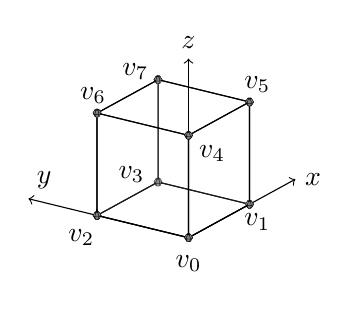
\begin{tikzpicture}[scale = 0.75, join=round]
\draw[arrows=<-,line width=.4pt](3.357,.613)--(2.621,.21);
\filldraw[fill=gray,line width=0.1pt](1.072,.587)--(1.052,.633)--(1.017,.633)--(1.002,.589)--cycle;
\filldraw[fill=gray,line width=0.1pt](1.017,.521)--(1.002,.589)--(.963,.567)--(.998,.51)--cycle;
\filldraw[fill=gray,line width=0.1pt](1.002,.589)--(1.017,.633)--(.998,.623)--(.963,.567)--cycle;
\filldraw[fill=gray,line width=0.1pt](1.052,.52)--(1.072,.587)--(1.002,.589)--(1.017,.521)--cycle;
\filldraw[fill=gray,line width=0.1pt](1.068,.509)--(1.102,.564)--(1.072,.587)--(1.052,.52)--cycle;
\filldraw[fill=gray,line width=0.1pt](1.102,.564)--(1.068,.621)--(1.052,.633)--(1.072,.587)--cycle;
\filldraw[fill=gray,line width=0.1pt](1.052,.52)--(1.013,.499)--(1.048,.498)--(1.017,.521)--cycle;
\filldraw[fill=gray,line width=0.1pt](1.048,.498)--(1.017,.521)--(.998,.51)--(1.068,.509)--cycle;
\filldraw[fill=gray,line width=0.1pt](.998,.51)--(1.068,.509)--(1.052,.52)--(1.013,.499)--cycle;
\filldraw[fill=gray,line width=0.1pt](.963,.567)--(.998,.51)--(1.013,.499)--(.994,.544)--cycle;
\filldraw[fill=gray,line width=0.1pt](1.064,.543)--(1.048,.498)--(1.068,.509)--(1.102,.564)--cycle;
\filldraw[fill=gray,line width=0.1pt](1.052,.633)--(1.013,.611)--(1.048,.611)--(1.017,.633)--cycle;
\filldraw[fill=gray,line width=0.1pt](1.017,.633)--(1.048,.611)--(1.068,.621)--(.998,.623)--cycle;
\filldraw[fill=gray,line width=0.1pt](1.068,.621)--(.998,.623)--(1.013,.611)--(1.052,.633)--cycle;
\filldraw[fill=gray,line width=0.1pt](.998,.623)--(.963,.567)--(.994,.544)--(1.013,.611)--cycle;
\filldraw[fill=gray,line width=0.1pt](.019,-.046)--(.039,.021)--(-.031,.023)--(-.015,-.045)--cycle;
\filldraw[fill=gray,line width=0.1pt](.039,.021)--(.019,.067)--(-.015,.068)--(-.031,.023)--cycle;
\draw[arrows=-,line width=.4pt](-.05,.012)--(-.101,.024);
\filldraw[fill=gray,line width=0.1pt](-.031,.023)--(-.015,.068)--(-.035,.057)--(-.07,.002)--cycle;
\filldraw[fill opacity=0.1,draw=none,fill=white](1.033,.622)--(1.033,.566)--(0,0)--(0,.166)--cycle;
\draw(1.033,.622)--(1.033,.566)--(0,0)--(0,.166);
\filldraw[fill=gray,draw=none](1.058,.616)--(1.083,.553)--(1.102,.564)--(1.068,.621)--cycle;
\draw[line width=0.1pt](1.083,.553)--(1.102,.564)--(1.068,.621)--(1.058,.616);
\filldraw[fill opacity=0.1,draw=none,fill=white](1.111,.61)--(1.083,.553)--(1.033,.566)--(1.033,.622)--cycle;
\draw(1.083,.553)--(1.033,.566)--(1.033,.622);
\filldraw[fill=gray,line width=0.1pt](.994,.544)--(1.013,.499)--(1.048,.498)--(1.064,.543)--cycle;
\filldraw[fill=gray,line width=0.1pt](2.601,.143)--(2.621,.21)--(2.551,.211)--(2.567,.144)--cycle;
\filldraw[fill=gray,draw=none](2.557,.138)--(2.567,.144)--(2.551,.211)--(2.532,.201)--cycle;
\draw[line width=0.1pt](2.557,.138)--(2.567,.144)--(2.551,.211)--(2.532,.201);
\filldraw[fill=gray,draw=none](2.557,.138)--(2.532,.201)--(2.512,.19)--(2.547,.133)--cycle;
\draw[line width=0.1pt](2.532,.201)--(2.512,.19)--(2.547,.133)--(2.557,.138);
\filldraw[fill=gray,line width=0.1pt](2.512,.19)--(2.547,.133)--(2.563,.122)--(2.543,.167)--cycle;
\filldraw[fill=gray,line width=0.1pt](.035,-.057)--(.07,-.002)--(.039,.021)--(.019,-.046)--cycle;
\filldraw[fill=gray,line width=0.1pt](.035,-.057)--(-.035,-.055)--(-.019,-.067)--(.019,-.046)--cycle;
\filldraw[fill=gray,draw=none](.05,-.012)--(.025,-.062)--(.035,-.057)--(.07,-.002)--cycle;
\draw[line width=0.1pt](.025,-.062)--(.035,-.057)--(.07,-.002)--(.05,-.012);
\filldraw[fill=gray,line width=0.1pt](1.569,-.423)--(1.588,-.356)--(1.518,-.354)--(1.534,-.422)--cycle;
\filldraw[fill=gray,draw=none](1.524,-.427)--(1.534,-.422)--(1.518,-.354)--(1.499,-.365)--cycle;
\draw[line width=0.1pt](1.524,-.427)--(1.534,-.422)--(1.518,-.354)--(1.499,-.365);
\filldraw[fill opacity=0.1,fill=white](1.033,.566)--(2.582,.189)--(1.549,-.377)--(0,0)--cycle;
\filldraw[fill=gray,line width=0.1pt](1.017,2.254)--(1.002,2.322)--(.963,2.301)--(.998,2.244)--cycle;
\filldraw[fill=gray,line width=0.1pt](1.052,2.253)--(1.072,2.32)--(1.002,2.322)--(1.017,2.254)--cycle;
\filldraw[fill=gray,draw=none](1.017,2.254)--(1.033,2.243)--(1.033,2.243)--(.998,2.244)--cycle;
\draw[line width=0.1pt](1.033,2.243)--(.998,2.244)--(1.017,2.254)--(1.033,2.243);
\filldraw[fill=gray,line width=0.1pt](.963,2.301)--(.998,2.244)--(1.013,2.232)--(.994,2.278)--cycle;
\filldraw[fill=gray,line width=0.1pt](.019,1.688)--(.039,1.755)--(-.031,1.756)--(-.015,1.688)--cycle;
\filldraw[fill opacity=0.1,draw=none,fill=white](1.033,2.299)--(1.033,.622)--(0,.166)--(0,1.733)--cycle;
\draw(0,.166)--(0,1.733)--(1.033,2.299)--(1.033,.622);
\filldraw[fill=gray,line width=0.1pt](1.068,2.242)--(1.102,2.297)--(1.072,2.32)--(1.052,2.253)--cycle;
\filldraw[fill=gray,draw=none](1.068,2.242)--(1.033,2.243)--(1.033,2.243)--(1.052,2.253)--cycle;
\draw[line width=0.1pt](1.033,2.243)--(1.052,2.253)--(1.068,2.242)--(1.033,2.243);
\filldraw[fill=gray,draw=none](1.033,2.243)--(1.058,2.237)--(1.068,2.242)--(1.033,2.243)--cycle;
\draw[line width=0.1pt](1.058,2.237)--(1.068,2.242)--(1.033,2.243);
\filldraw[fill=gray,draw=none](1.083,2.287)--(1.058,2.237)--(1.068,2.242)--(1.102,2.297)--cycle;
\draw[line width=0.1pt](1.058,2.237)--(1.068,2.242)--(1.102,2.297)--(1.083,2.287);
\filldraw[fill opacity=0.1,draw=none,fill=white](1.111,.61)--(1.033,.622)--(1.033,2.299)--(1.858,2.098)--cycle;
\draw(1.033,.622)--(1.033,2.299)--(1.858,2.098);
\filldraw[fill=gray,draw=none](2.532,.201)--(2.551,.211)--(2.567,.256)--(2.557,.251)--cycle;
\draw[line width=0.1pt](2.532,.201)--(2.551,.211)--(2.567,.256)--(2.557,.251);
\filldraw[fill=gray,line width=0.1pt](2.621,.21)--(2.601,.255)--(2.567,.256)--(2.551,.211)--cycle;
\filldraw[fill=gray,line width=0.1pt](2.652,.187)--(2.617,.244)--(2.601,.255)--(2.621,.21)--cycle;
\filldraw[fill=gray,draw=none](2.557,.251)--(2.567,.256)--(2.582,.245)--(2.607,.239)--(2.617,.244)--(2.582,.245)--cycle;
\draw[line width=0.1pt](2.557,.251)--(2.567,.256)--(2.582,.245);
\draw[line width=0.1pt](2.607,.239)--(2.617,.244)--(2.582,.245);
\filldraw[fill=gray,draw=none](2.557,1.872)--(2.567,1.877)--(2.551,1.945)--(2.532,1.934)--cycle;
\draw[line width=0.1pt](2.557,1.872)--(2.567,1.877)--(2.551,1.945)--(2.532,1.934);
\filldraw[fill=gray,line width=0.1pt](2.601,1.876)--(2.621,1.943)--(2.551,1.945)--(2.567,1.877)--cycle;
\filldraw[fill opacity=0.1,draw=none,fill=white](1.083,.553)--(1.858,2.098)--(2.582,1.922)--(2.582,.189)--cycle;
\draw(1.858,2.098)--(2.582,1.922)--(2.582,.189)--(1.083,.553);
\filldraw[fill=gray,draw=none](1.058,.616)--(1.048,.611)--(1.064,.543)--(1.083,.553)--cycle;
\draw[line width=0.1pt](1.058,.616)--(1.048,.611)--(1.064,.543)--(1.083,.553);
\filldraw[fill=gray,line width=0.1pt](1.013,.611)--(.994,.544)--(1.064,.543)--(1.048,.611)--cycle;
\filldraw[fill=gray,line width=0.1pt](1.002,2.322)--(1.017,2.367)--(.998,2.356)--(.963,2.301)--cycle;
\filldraw[fill=gray,line width=0.1pt](1.072,2.32)--(1.052,2.366)--(1.017,2.367)--(1.002,2.322)--cycle;
\filldraw[fill=gray,line width=0.1pt](1.102,2.297)--(1.068,2.354)--(1.052,2.366)--(1.072,2.32)--cycle;
\filldraw[fill=gray,line width=0.1pt](1.052,2.253)--(1.013,2.232)--(1.048,2.231)--(1.017,2.254)--cycle;
\filldraw[fill=gray,draw=none](1.033,2.243)--(.998,2.244)--(1.013,2.232)--(1.033,2.243)--cycle;
\draw[line width=0.1pt](1.033,2.243)--(.998,2.244)--(1.013,2.232)--(1.033,2.243);
\filldraw[fill=gray,draw=none](1.033,2.243)--(1.048,2.231)--(1.058,2.237)--(1.033,2.243)--cycle;
\draw[line width=0.1pt](1.033,2.243)--(1.048,2.231)--(1.058,2.237);
\filldraw[fill=gray,line width=0.1pt](1.052,2.366)--(1.013,2.345)--(1.048,2.344)--(1.017,2.367)--cycle;
\filldraw[fill=gray,line width=0.1pt](1.048,2.344)--(1.017,2.367)--(.998,2.356)--(1.068,2.354)--cycle;
\filldraw[fill=gray,draw=none](1.083,2.287)--(1.064,2.276)--(1.048,2.231)--(1.058,2.237)--cycle;
\draw[line width=0.1pt](1.083,2.287)--(1.064,2.276)--(1.048,2.231)--(1.058,2.237);
\filldraw[fill=gray,line width=0.1pt](.998,2.356)--(1.068,2.354)--(1.052,2.366)--(1.013,2.345)--cycle;
\filldraw[fill=gray,line width=0.1pt](.998,2.356)--(.963,2.301)--(.994,2.278)--(1.013,2.345)--cycle;
\filldraw[fill=gray,line width=0.1pt](.994,2.278)--(1.013,2.232)--(1.048,2.231)--(1.064,2.276)--cycle;
\filldraw[fill=gray,draw=none](2.557,1.872)--(2.532,1.934)--(2.512,1.924)--(2.547,1.866)--cycle;
\draw[line width=0.1pt](2.532,1.934)--(2.512,1.924)--(2.547,1.866)--(2.557,1.872);
\filldraw[fill=gray,draw=none](2.567,1.877)--(2.582,1.866)--(2.582,1.866)--(2.547,1.866)--cycle;
\draw[line width=0.1pt](2.582,1.866)--(2.547,1.866)--(2.567,1.877)--(2.582,1.866);
\filldraw[fill=gray,line width=0.1pt](2.512,1.924)--(2.547,1.866)--(2.563,1.855)--(2.543,1.901)--cycle;
\filldraw[fill=gray,line width=0.1pt](.035,1.676)--(.07,1.732)--(.039,1.755)--(.019,1.688)--cycle;
\filldraw[fill=gray,draw=none](.035,1.676)--(0,1.677)--(0,1.677)--(.019,1.688)--cycle;
\draw[line width=0.1pt](0,1.677)--(.019,1.688)--(.035,1.676)--(0,1.677);
\filldraw[fill=gray,draw=none](0,1.677)--(.035,1.676)--(.019,1.688)--(0,1.677)--cycle;
\draw[line width=0.1pt](0,1.677)--(.035,1.676)--(.019,1.688)--(0,1.677);
\filldraw[fill=gray,draw=none](.05,1.721)--(.025,1.671)--(.035,1.676)--(.07,1.732)--cycle;
\draw[line width=0.1pt](.025,1.671)--(.035,1.676)--(.07,1.732)--(.05,1.721);
\filldraw[fill=gray,draw=none](1.524,1.306)--(1.534,1.311)--(1.518,1.379)--(1.499,1.368)--cycle;
\draw[line width=0.1pt](1.524,1.306)--(1.534,1.311)--(1.518,1.379)--(1.499,1.368);
\filldraw[fill=gray,line width=0.1pt](1.569,1.311)--(1.588,1.377)--(1.518,1.379)--(1.534,1.311)--cycle;
\filldraw[fill opacity=0.1,fill=white](2.582,1.922)--(1.033,2.299)--(0,1.733)--(1.549,1.356)--cycle;
\filldraw[fill=gray,draw=none](1.058,2.349)--(1.083,2.287)--(1.102,2.297)--(1.068,2.354)--cycle;
\draw[line width=0.1pt](1.083,2.287)--(1.102,2.297)--(1.068,2.354)--(1.058,2.349);
\filldraw[fill=gray,draw=none](1.058,2.349)--(1.048,2.344)--(1.064,2.276)--(1.083,2.287)--cycle;
\draw[line width=0.1pt](1.058,2.349)--(1.048,2.344)--(1.064,2.276)--(1.083,2.287);
\draw[arrows=->,line width=.4pt](-.101,.024)--(-1.162,.283);
\filldraw[fill=gray,line width=0.1pt](1.013,2.345)--(.994,2.278)--(1.064,2.276)--(1.048,2.344)--cycle;
\draw[arrows=-,line width=.4pt](2.621,.21)--(2.543,.167);
\filldraw[fill=gray,line width=0.1pt](2.617,.131)--(2.652,.187)--(2.621,.21)--(2.601,.143)--cycle;
\filldraw[fill=gray,line width=0.1pt](2.601,.143)--(2.563,.122)--(2.597,.121)--(2.567,.144)--cycle;
\filldraw[fill=gray,line width=0.1pt](2.597,.121)--(2.567,.144)--(2.547,.133)--(2.617,.131)--cycle;
\filldraw[fill=gray,line width=0.1pt](2.563,.122)--(2.601,.143)--(2.567,.144)--(2.597,.121)--cycle;
\filldraw[fill=gray,line width=0.1pt](2.617,.131)--(2.547,.133)--(2.563,.122)--(2.601,.143)--cycle;
\filldraw[fill=gray,line width=0.1pt](2.547,.133)--(2.617,.131)--(2.601,.143)--(2.563,.122)--cycle;
\filldraw[fill=gray,draw=none](2.532,.201)--(2.557,.251)--(2.547,.246)--(2.512,.19)--cycle;
\draw[line width=0.1pt](2.557,.251)--(2.547,.246)--(2.512,.19)--(2.532,.201);
\filldraw[fill=gray,line width=0.1pt](2.613,.166)--(2.597,.121)--(2.617,.131)--(2.652,.187)--cycle;
\filldraw[fill=gray,line width=0.1pt](2.563,.234)--(2.601,.255)--(2.567,.256)--(2.597,.233)--cycle;
\filldraw[fill=gray,draw=none](2.582,.245)--(2.617,.244)--(2.601,.255)--(2.582,.245)--cycle;
\draw[line width=0.1pt](2.582,.245)--(2.617,.244)--(2.601,.255)--(2.582,.245);
\filldraw[fill=gray,line width=0.1pt](2.547,.246)--(2.512,.19)--(2.543,.167)--(2.563,.234)--cycle;
\filldraw[fill=gray,draw=none](2.557,.251)--(2.582,.245)--(2.597,.233)--(2.607,.239)--(2.582,.245)--(2.547,.246)--cycle;
\draw[line width=0.1pt](2.582,.245)--(2.597,.233)--(2.607,.239);
\draw[line width=0.1pt](2.582,.245)--(2.547,.246)--(2.557,.251);
\filldraw[fill=gray,draw=none](2.547,.246)--(2.582,.245)--(2.582,.245)--(2.563,.234)--cycle;
\draw[line width=0.1pt](2.582,.245)--(2.563,.234)--(2.547,.246)--(2.582,.245);
\filldraw[fill=gray,line width=0.1pt](1.588,-.356)--(1.569,-.31)--(1.534,-.309)--(1.518,-.354)--cycle;
\filldraw[fill opacity=0.1,fill=white](2.582,.189)--(2.582,1.922)--(1.549,1.356)--(1.549,-.377)--cycle;
\filldraw[fill=gray,line width=0.1pt](2.597,.233)--(2.613,.166)--(2.652,.187)--(2.617,.244)--cycle;
\filldraw[fill=gray,line width=0.1pt](2.543,.167)--(2.563,.122)--(2.597,.121)--(2.613,.166)--cycle;
\filldraw[fill=gray,line width=0.1pt](2.563,.234)--(2.543,.167)--(2.613,.166)--(2.597,.233)--cycle;
\draw[arrows=-,line width=.4pt](2.543,.167)--(2.184,-.029);
\filldraw[fill=gray,line width=0.1pt](-.015,-.045)--(-.031,.023)--(-.07,.002)--(-.035,-.055)--cycle;
\filldraw[fill=gray,line width=0.1pt](.07,-.002)--(.035,.055)--(.019,.067)--(.039,.021)--cycle;
\filldraw[fill=gray,line width=0.1pt](.015,-.068)--(-.015,-.045)--(-.035,-.055)--(.035,-.057)--cycle;
\filldraw[fill=gray,line width=0.1pt](.019,-.046)--(-.019,-.067)--(.015,-.068)--(-.015,-.045)--cycle;
\filldraw[fill=gray,line width=0.1pt](-.015,-.045)--(.015,-.068)--(.035,-.057)--(-.035,-.055)--cycle;
\filldraw[fill=gray,line width=0.1pt](-.019,-.067)--(.019,-.046)--(-.015,-.045)--(.015,-.068)--cycle;
\filldraw[fill=gray,line width=0.1pt](-.035,-.055)--(.035,-.057)--(.019,-.046)--(-.019,-.067)--cycle;
\draw[arrows=-,line width=.4pt](.05,-.012)--(-.05,.012);
\filldraw[fill=gray,line width=0.1pt](-.07,.002)--(-.035,-.055)--(-.019,-.067)--(-.039,-.021)--cycle;
\filldraw[fill=gray,draw=none](0,.056)--(0,.056)--(.019,.067)--cycle;
\draw[line width=0.1pt](0,.056)--(.019,.067);
\filldraw[fill=gray,draw=none](.035,.055)--(0,.056)--(-.019,.046)--(.019,.067)--cycle;
\draw[line width=0.1pt](-.019,.046)--(.019,.067)--(.035,.055)--(0,.056);
\filldraw[fill=gray,draw=none](0,.056)--(.019,.067)--(0,.056)--cycle;
\draw[line width=0.1pt](.019,.067)--(0,.056);
\filldraw[fill=gray,draw=none](0,.056)--(.035,.055)--(.019,.067)--(-.019,.046)--cycle;
\draw[line width=0.1pt](0,.056)--(.035,.055)--(.019,.067)--(-.019,.046);
\filldraw[fill=gray,line width=0.1pt](-.019,.046)--(.019,.067)--(-.015,.068)--(.015,.045)--cycle;
\filldraw[fill=gray,draw=none](.05,-.012)--(.031,-.023)--(.015,-.068)--(.025,-.062)--cycle;
\draw[line width=0.1pt](.05,-.012)--(.031,-.023)--(.015,-.068)--(.025,-.062);
\filldraw[fill=gray,line width=0.1pt](-.035,.057)--(-.07,.002)--(-.039,-.021)--(-.019,.046)--cycle;
\filldraw[fill=gray,draw=none](.025,.05)--(.05,-.012)--(.07,-.002)--(.035,.055)--cycle;
\draw[line width=0.1pt](.05,-.012)--(.07,-.002)--(.035,.055)--(.025,.05);
\filldraw[fill=gray,draw=none](1.499,-.365)--(1.518,-.354)--(1.534,-.309)--(1.524,-.315)--cycle;
\draw[line width=0.1pt](1.499,-.365)--(1.518,-.354)--(1.534,-.309)--(1.524,-.315);
\draw[arrows=-,line width=.4pt](2.184,-.029)--(1.588,-.356);
\filldraw[fill=gray,line width=0.1pt](1.619,-.379)--(1.584,-.322)--(1.569,-.31)--(1.588,-.356)--cycle;
\filldraw[fill=gray,line width=0.1pt](1.565,-.332)--(1.534,-.309)--(1.514,-.32)--(1.584,-.322)--cycle;
\filldraw[fill opacity=0.1,draw=none,fill=white](1.549,-.377)--(1.549,-.321)--(0,.056)--(0,0)--cycle;
\draw(0,.056)--(0,0)--(1.549,-.377)--(1.549,-.321);
\filldraw[fill=gray,line width=0.1pt](-.039,-.021)--(-.019,-.067)--(.015,-.068)--(.031,-.023)--cycle;
\filldraw[fill=gray,draw=none](0,.056)--(-.035,.057)--(-.019,.046)--(0,.056)--cycle;
\draw[line width=0.1pt](0,.056)--(-.035,.057)--(-.019,.046)--(0,.056);
\filldraw[fill=gray,draw=none](-.035,.057)--(0,.056)--(0,.056)--(-.019,.046)--cycle;
\draw[line width=0.1pt](0,.056)--(-.019,.046)--(-.035,.057)--(0,.056);
\filldraw[fill opacity=0.1,draw=none,fill=white](.025,.05)--(0,.113)--(0,.056)--cycle;
\draw(0,.113)--(0,.056);
\draw[arrows=-,line width=.4pt](.101,-.024)--(.05,-.012);
\filldraw[fill=gray,draw=none](.025,.05)--(.015,.045)--(.031,-.023)--(.05,-.012)--cycle;
\draw[line width=0.1pt](.025,.05)--(.015,.045)--(.031,-.023)--(.05,-.012);
\filldraw[fill=gray,draw=none](0,1.677)--(0,1.677)--(.019,1.688)--cycle;
\draw[line width=0.1pt](0,1.677)--(.019,1.688);
\filldraw[fill=gray,draw=none](0,1.677)--(.019,1.688)--(0,1.677)--cycle;
\draw[line width=0.1pt](.019,1.688)--(0,1.677);
\filldraw[fill=gray,draw=none](1.549,1.3)--(1.534,1.311)--(1.524,1.306)--(1.549,1.3)--cycle;
\draw[line width=0.1pt](1.549,1.3)--(1.534,1.311)--(1.524,1.306);
\filldraw[fill opacity=0.1,draw=none,fill=white](.025,.05)--(1.549,-.321)--(1.549,1.356)--(0,1.733)--(0,.113)--cycle;
\draw(1.549,-.321)--(1.549,1.356)--(0,1.733)--(0,.113);
\filldraw[fill=gray,line width=0.1pt](-.019,.046)--(-.039,-.021)--(.031,-.023)--(.015,.045)--cycle;
\draw[arrows=-,line width=.4pt](1.449,-.353)--(.101,-.024);
\filldraw[fill=gray,draw=none](2.532,1.934)--(2.551,1.945)--(2.567,1.99)--(2.557,1.984)--cycle;
\draw[line width=0.1pt](2.532,1.934)--(2.551,1.945)--(2.567,1.99)--(2.557,1.984);
\filldraw[fill=gray,line width=0.1pt](2.621,1.943)--(2.601,1.989)--(2.567,1.99)--(2.551,1.945)--cycle;
\filldraw[fill=gray,line width=0.1pt](2.617,1.865)--(2.652,1.92)--(2.621,1.943)--(2.601,1.876)--cycle;
\filldraw[fill=gray,line width=0.1pt](2.652,1.92)--(2.617,1.977)--(2.601,1.989)--(2.621,1.943)--cycle;
\filldraw[fill=gray,line width=0.1pt](2.563,1.855)--(2.601,1.876)--(2.567,1.877)--(2.597,1.854)--cycle;
\filldraw[fill=gray,line width=0.1pt](2.617,1.865)--(2.547,1.866)--(2.563,1.855)--(2.601,1.876)--cycle;
\filldraw[fill=gray,draw=none](2.532,1.934)--(2.557,1.984)--(2.547,1.979)--(2.512,1.924)--cycle;
\draw[line width=0.1pt](2.557,1.984)--(2.547,1.979)--(2.512,1.924)--(2.532,1.934);
\filldraw[fill=gray,draw=none](2.582,1.866)--(2.597,1.854)--(2.617,1.865)--(2.582,1.866)--cycle;
\draw[line width=0.1pt](2.582,1.866)--(2.597,1.854)--(2.617,1.865)--(2.582,1.866);
\filldraw[fill=gray,line width=0.1pt](2.613,1.899)--(2.597,1.854)--(2.617,1.865)--(2.652,1.92)--cycle;
\filldraw[fill=gray,line width=0.1pt](2.563,1.968)--(2.601,1.989)--(2.567,1.99)--(2.597,1.967)--cycle;
\filldraw[fill=gray,line width=0.1pt](2.597,1.967)--(2.567,1.99)--(2.547,1.979)--(2.617,1.977)--cycle;
\filldraw[fill=gray,line width=0.1pt](2.547,1.979)--(2.617,1.977)--(2.601,1.989)--(2.563,1.968)--cycle;
\filldraw[fill=gray,line width=0.1pt](2.617,1.977)--(2.547,1.979)--(2.563,1.968)--(2.601,1.989)--cycle;
\filldraw[fill=gray,line width=0.1pt](2.547,1.979)--(2.512,1.924)--(2.543,1.901)--(2.563,1.968)--cycle;
\filldraw[fill=gray,line width=0.1pt](2.597,1.967)--(2.613,1.899)--(2.652,1.92)--(2.617,1.977)--cycle;
\filldraw[fill=gray,line width=0.1pt](2.543,1.901)--(2.563,1.855)--(2.597,1.854)--(2.613,1.899)--cycle;
\filldraw[fill=gray,line width=0.1pt](2.563,1.968)--(2.543,1.901)--(2.613,1.899)--(2.597,1.967)--cycle;
\filldraw[fill=gray,line width=0.1pt](.039,1.755)--(.019,1.8)--(-.015,1.801)--(-.031,1.756)--cycle;
\filldraw[fill=gray,line width=0.1pt](-.015,1.688)--(-.031,1.756)--(-.07,1.735)--(-.035,1.678)--cycle;
\filldraw[fill=gray,line width=0.1pt](-.031,1.756)--(-.015,1.801)--(-.035,1.79)--(-.07,1.735)--cycle;
\filldraw[fill=gray,line width=0.1pt](.07,1.732)--(.035,1.789)--(.019,1.8)--(.039,1.755)--cycle;
\filldraw[fill=gray,line width=0.1pt](.019,1.688)--(-.019,1.666)--(.015,1.666)--(-.015,1.688)--cycle;
\filldraw[fill=gray,draw=none](0,1.677)--(-.035,1.678)--(-.019,1.666)--(0,1.677)--cycle;
\draw[line width=0.1pt](0,1.677)--(-.035,1.678)--(-.019,1.666)--(0,1.677);
\filldraw[fill=gray,draw=none](-.035,1.678)--(0,1.677)--(0,1.677)--(-.019,1.666)--cycle;
\draw[line width=0.1pt](0,1.677)--(-.019,1.666)--(-.035,1.678)--(0,1.677);
\filldraw[fill=gray,line width=0.1pt](-.07,1.735)--(-.035,1.678)--(-.019,1.666)--(-.039,1.712)--cycle;
\filldraw[fill=gray,draw=none](0,1.677)--(0,1.677)--(-.019,1.666)--cycle;
\draw[line width=0.1pt](0,1.677)--(-.019,1.666);
\filldraw[fill=gray,draw=none](0,1.677)--(-.019,1.666)--(0,1.677)--cycle;
\draw[line width=0.1pt](-.019,1.666)--(0,1.677);
\filldraw[fill=gray,line width=0.1pt](.019,1.8)--(-.019,1.779)--(.015,1.778)--(-.015,1.801)--cycle;
\filldraw[fill=gray,line width=0.1pt](-.015,1.801)--(.015,1.778)--(.035,1.789)--(-.035,1.79)--cycle;
\filldraw[fill=gray,draw=none](.05,1.721)--(.031,1.71)--(.015,1.666)--(.025,1.671)--cycle;
\draw[line width=0.1pt](.05,1.721)--(.031,1.71)--(.015,1.666)--(.025,1.671);
\filldraw[fill=gray,line width=0.1pt](-.035,1.79)--(.035,1.789)--(.019,1.8)--(-.019,1.779)--cycle;
\filldraw[fill=gray,line width=0.1pt](.035,1.789)--(-.035,1.79)--(-.019,1.779)--(.019,1.8)--cycle;
\filldraw[fill=gray,line width=0.1pt](-.035,1.79)--(-.07,1.735)--(-.039,1.712)--(-.019,1.779)--cycle;
\filldraw[fill=gray,draw=none](.025,1.784)--(.05,1.721)--(.07,1.732)--(.035,1.789)--cycle;
\draw[line width=0.1pt](.05,1.721)--(.07,1.732)--(.035,1.789)--(.025,1.784);
\filldraw[fill=gray,line width=0.1pt](-.039,1.712)--(-.019,1.666)--(.015,1.666)--(.031,1.71)--cycle;
\filldraw[fill=gray,draw=none](.025,1.784)--(.015,1.778)--(.031,1.71)--(.05,1.721)--cycle;
\draw[line width=0.1pt](.025,1.784)--(.015,1.778)--(.031,1.71)--(.05,1.721);
\filldraw[fill=gray,line width=0.1pt](-.019,1.779)--(-.039,1.712)--(.031,1.71)--(.015,1.778)--cycle;
\draw[arrows=-,line width=.4pt](1.499,-.365)--(1.449,-.353);
\draw[arrows=-,line width=.4pt](1.588,-.356)--(1.549,-.377)--(1.499,-.365);
\filldraw[fill=gray,line width=0.1pt](1.584,-.434)--(1.619,-.379)--(1.588,-.356)--(1.569,-.423)--cycle;
\filldraw[fill=gray,line width=0.1pt](1.534,-.422)--(1.565,-.445)--(1.584,-.434)--(1.514,-.433)--cycle;
\filldraw[fill=gray,line width=0.1pt](1.569,-.423)--(1.53,-.444)--(1.565,-.445)--(1.534,-.422)--cycle;
\filldraw[fill=gray,line width=0.1pt](1.565,-.445)--(1.534,-.422)--(1.514,-.433)--(1.584,-.434)--cycle;
\filldraw[fill=gray,draw=none](1.524,-.427)--(1.499,-.365)--(1.48,-.375)--(1.514,-.433)--cycle;
\draw[line width=0.1pt](1.499,-.365)--(1.48,-.375)--(1.514,-.433)--(1.524,-.427);
\filldraw[fill=gray,draw=none](1.499,-.365)--(1.524,-.315)--(1.514,-.32)--(1.48,-.375)--cycle;
\draw[line width=0.1pt](1.524,-.315)--(1.514,-.32)--(1.48,-.375)--(1.499,-.365);
\filldraw[fill=gray,line width=0.1pt](1.48,-.375)--(1.514,-.433)--(1.53,-.444)--(1.51,-.398)--cycle;
\filldraw[fill=gray,line width=0.1pt](1.58,-.4)--(1.565,-.445)--(1.584,-.434)--(1.619,-.379)--cycle;
\filldraw[fill=gray,line width=0.1pt](1.534,-.309)--(1.565,-.332)--(1.584,-.322)--(1.514,-.32)--cycle;
\filldraw[fill=gray,line width=0.1pt](1.53,-.331)--(1.569,-.31)--(1.534,-.309)--(1.565,-.332)--cycle;
\filldraw[fill=gray,draw=none](1.549,-.321)--(1.569,-.31)--(1.549,-.321)--cycle;
\draw[line width=0.1pt](1.569,-.31)--(1.549,-.321);
\filldraw[fill=gray,draw=none](1.549,-.321)--(1.584,-.322)--(1.569,-.31)--(1.53,-.331)--cycle;
\draw[line width=0.1pt](1.549,-.321)--(1.584,-.322)--(1.569,-.31)--(1.53,-.331);
\filldraw[fill=gray,line width=0.1pt](1.514,-.32)--(1.48,-.375)--(1.51,-.398)--(1.53,-.331)--cycle;
\draw[arrows=-,line width=.4pt](1.549,-.377)--(1.549,-.321);
\filldraw[fill=gray,line width=0.1pt](1.565,-.332)--(1.58,-.4)--(1.619,-.379)--(1.584,-.322)--cycle;
\filldraw[fill=gray,line width=0.1pt](1.51,-.398)--(1.53,-.444)--(1.565,-.445)--(1.58,-.4)--cycle;
\filldraw[fill=gray,draw=none](1.514,-.32)--(1.549,-.321)--(1.549,-.321)--(1.53,-.331)--cycle;
\draw[line width=0.1pt](1.549,-.321)--(1.53,-.331)--(1.514,-.32)--(1.549,-.321);
\draw[arrows=-,line width=.4pt](1.549,-.321)--(1.549,1.244);
\filldraw[fill=gray,line width=0.1pt](1.53,-.331)--(1.51,-.398)--(1.58,-.4)--(1.565,-.332)--cycle;
\filldraw[fill=gray,draw=none](1.499,1.368)--(1.518,1.379)--(1.534,1.424)--(1.524,1.419)--cycle;
\draw[line width=0.1pt](1.499,1.368)--(1.518,1.379)--(1.534,1.424)--(1.524,1.419);
\filldraw[fill=gray,line width=0.1pt](1.588,1.377)--(1.569,1.423)--(1.534,1.424)--(1.518,1.379)--cycle;
\filldraw[fill=gray,line width=0.1pt](1.584,1.299)--(1.619,1.355)--(1.588,1.377)--(1.569,1.311)--cycle;
\filldraw[fill=gray,line width=0.1pt](1.619,1.355)--(1.584,1.412)--(1.569,1.423)--(1.588,1.377)--cycle;
\filldraw[fill=gray,line width=0.1pt](1.569,1.311)--(1.53,1.289)--(1.565,1.288)--(1.534,1.311)--cycle;
\draw[arrows=-,line width=.4pt](1.549,1.244)--(1.549,1.356);
\filldraw[fill=gray,draw=none](1.549,1.3)--(1.524,1.306)--(1.514,1.301)--(1.549,1.3)--cycle;
\draw[line width=0.1pt](1.524,1.306)--(1.514,1.301)--(1.549,1.3);
\filldraw[fill=gray,draw=none](1.524,1.306)--(1.499,1.368)--(1.48,1.358)--(1.514,1.301)--cycle;
\draw[line width=0.1pt](1.499,1.368)--(1.48,1.358)--(1.514,1.301)--(1.524,1.306);
\filldraw[fill=gray,draw=none](1.499,1.368)--(1.524,1.419)--(1.514,1.413)--(1.48,1.358)--cycle;
\draw[line width=0.1pt](1.524,1.419)--(1.514,1.413)--(1.48,1.358)--(1.499,1.368);
\filldraw[fill=gray,line width=0.1pt](1.48,1.358)--(1.514,1.301)--(1.53,1.289)--(1.51,1.335)--cycle;
\filldraw[fill=gray,draw=none](1.574,1.294)--(1.565,1.288)--(1.549,1.3)--(1.549,1.3)--cycle;
\draw[line width=0.1pt](1.574,1.294)--(1.565,1.288)--(1.549,1.3);
\filldraw[fill=gray,draw=none](1.574,1.294)--(1.549,1.3)--(1.549,1.3)--(1.584,1.299)--cycle;
\draw[line width=0.1pt](1.549,1.3)--(1.584,1.299)--(1.574,1.294);
\filldraw[fill=gray,line width=0.1pt](1.58,1.333)--(1.565,1.288)--(1.584,1.299)--(1.619,1.355)--cycle;
\filldraw[fill=gray,line width=0.1pt](1.569,1.423)--(1.53,1.402)--(1.565,1.401)--(1.534,1.424)--cycle;
\filldraw[fill=gray,line width=0.1pt](1.514,1.413)--(1.48,1.358)--(1.51,1.335)--(1.53,1.402)--cycle;
\draw[arrows=-,line width=.4pt](1.549,1.356)--(1.549,1.469);
\filldraw[fill=gray,line width=0.1pt](1.565,1.401)--(1.58,1.333)--(1.619,1.355)--(1.584,1.412)--cycle;
\filldraw[fill=gray,line width=0.1pt](1.51,1.335)--(1.53,1.289)--(1.565,1.288)--(1.58,1.333)--cycle;
\draw[arrows=->,line width=.4pt](1.549,1.469)--(1.549,2.656);
\filldraw[fill=gray,line width=0.1pt](1.53,1.402)--(1.51,1.335)--(1.58,1.333)--(1.565,1.401)--cycle;
\path (1.549,2.656) node[above] {$z$}
                   (3.357,.613) node[right] {$x$}
                   (-1.162,.283) node[above, xshift=2mm] {$y$};
\path (0,0) node[below, xshift=-2mm, yshift=-0.5mm] {$v_2$}
			(1.549,-.377) node[below, yshift=-1mm] {$v_0$}                  
                  (1.033,.566) node[left, xshift=-0.5mm, yshift=1mm] {$v_3$}
			(2.582,.189) node[below, xshift=1mm] {$v_1$}
			(0,1.733) node[above, xshift=-0.5mm] {$v_6$}                  
                  (1.549,1.356) node[below, xshift=3mm] {$v_4$}
                  (1.033,2.299) node[left, yshift=1mm] {$v_7$}
			(2.582,1.922) node[above, xshift=1mm] {$v_5$};
\end{tikzpicture}
%\end{center}
%\vspace*{\fill}
%\end{document}
% End sketch output
 } 
  \subfigure[Child 2]{
   \label{fig:child2}
  \input{figures/child2} } 
  \subfigure[Child 3 ]{
   \label{fig:child3}
  \input{figures/child3} }     
  \subfigure[Child 4]{
   \label{fig:child4}
  \input{figures/child4} } 
  \subfigure[Child 5]{
   \label{fig:child5}
  \input{figures/child5} }
  \subfigure[Child 6]{
   \label{fig:child6}
  \input{figures/child6} }
  \subfigure[Child 7]{
   \label{fig:child7}
  \input{figures/child7} }
  \caption{Local coordinate systems for each of the 8 child number configurations. In each of these configurations, $v_0$ is the node that this element shares with its parent and $v_7$ is the node that this element shares with all its siblings. For an element with child number $k$, $v_0$ will be the k-th node and $v_7$ will be the (7-k)-th node. $v_0$ and $v_7$ can never be hanging. If $v_3$, $v_5$ or $v_6$ are hanging, they will be face-hanging and not edge-hanging. If $v_3$ is hanging, then $v_1$ and $v_2$ must be edge-hanging. If $v_5$ is hanging, then $v_1$ and $v_4$ must be edge-hanging. If $v_6$ is hanging, then $v_2$ and $v_4$ must be edge-hanging.} 
  \end {center}
\end{figure}

At present, DENDRO only supports trilinear lagrange shape functions. The salient differences between the shape functions for regular grids and those for the DENDRO framework are the following.
\begin{enumerate}
\item There are no shape functions rooted at the hanging nodes. 
\item The support of a shape function can spread over more than 8 elements.
\item If a node of an element is hanging, then the shape functions rooted at the other regular nodes in that element do not vanish on this hanging node. Instead, they will vanish at the regular node that this hanging node is mapped to. For example, in Figure \ref{fig:hanging} the shape function rooted at node $a_0$ will not vanish at nodes $a_1$, $a_2$, $a_3$, $a_4$, $a_5$ or $a_6$. It will vanish at nodes $p_1$, $p_2$, $p_3$, $p_4$, $p_5$, $p_6$ and $a_7$. It will assume a value equal to 1 at node $a_0$.
\end{enumerate}

One could pre-compute the finite element stencils for all the 8x18 element types. While doing this, it is best if one uses the same numbering convention as is used within DENDRO (Table \ref{tab:etypes}).  Alternatively, one could just pre-compute the stencils for a specific child number configuration, e.g. child 0 and use rotations to compute the stencils for the other types on the fly inside the matvec. In this case, it will be useful to work with the following two types of coordinate systems:
\begin{enumerate}
\item The global coordinate system, which is also the local coordinate system for elements with child number 0. DENDRO consistently uses the global coordinate system in all its functions. 
\item The local coordinate system of an element depends on its child number. For an octant with child number equal to 'k', the local coordinate system is simply defined as a right handed coordinate system with origin at node 'k' and oriented so that the node $(7-k)$ is facing in the +x,+y,+z directions (in the local coordinate system) from the origin (node 'k'). Figures \ref{fig:child0} - \ref{fig:child7} illustrates the local coordinates systems for each of the 8 'child number' configurations. 
\end{enumerate}

The stencils can be compressed further if the differential operator under consideration is invariant under a cyclic rotation of the coordinates, i.e. ($x \leftarrow y$, $y \leftarrow z$, $z \leftarrow x$). In this case, it is not even necessary to pre-compute the stencils for all the 18 different hanging node configurations. For example, the scalar laplacian only needs 8 different types of stencils, the stencils for the remaining types can be derived using simple linear transformations. We will not discuss these transformations here. 

\section{Constructing the finite element mesh}
\label{sec:daconstructor}
The finite element mesh is constructed by calling the constructor of the class ot::DA. This will create the element-to-node mappings and will set up the scatter contexts used for communicating ghost values inside the matvecs. If you want to use the multigrid solver, then there is no need to call this constructor explicitly. While setting up the multigrid context, this constructor will be called internally for each level.

\section{Creating a PETSc Mat object using ot::DA}
\label{sec:matcreate}
DENDRO provides the following functions to query for the number of nodes and/or elements owned by each processor. This information is sufficient to create any of the Matrix types supported by PETSc. Refer the PETSc manual to learn about the various matrix types and how to create them.

Use the following functions to get the number of nodes and elements owned by the calling processor.

\begin{lstlisting}[frame=trbl, fontadjust]{}
unsigned int ot::DA::getNodeSize()
unsigned int ot::DA:getElementSize()
\end{lstlisting}

To get the sizes including ghosts as well use the following functions:

\begin{lstlisting}[frame=trbl, fontadjust]{}
unsigned int ot::DA::getGhostedNodeSize()
unsigned int ot::DA::getGhostedElementSize()
\end{lstlisting}

Since, most FEM matrices will have a local size equal to the local node size on each processor, DENDRO provides a wrapper for this type of matrices. This is listed below:

\begin{lstlisting}[frame=trbl, fontadjust]{}
int ot::DA::createMatrix(Mat& M, MatType mtype, unsigned int dof = 1)
\end{lstlisting}
The local size of the matrix will be (dof $\times$ ot::DA::getNodeSize()). Use the function \lstinline[basicstyle=\bfseries]!createActiveMatrix()! instead to create a matrix
 that is distributed only on the active processors.

One should not set the matrix entries directly using the functions provided in PETSc. This will not be possible as the indexing used by PETSc is different from that used in DENDRO. Section \ref{sec:matassemble} describes how to set values into a matrix using DENDRO.

\section{Creating a PETSc 'Vec' object using ot::DA}
\label{sec:petscveccreate}
One can query DENDRO for the local sizes using the functions described in Section \ref{sec:matcreate} and use them to create PETSc vectors as described in the PETSc manual. Alternatively, one can use the following wrapper provided in DENDRO.

\begin{lstlisting}[frame=trbl, fontadjust]{}
int createVector(Vec & local, bool isElemental,
 bool isGhosted, unsigned int dof = 1)
\end{lstlisting}

Use the function \lstinline[basicstyle=\bfseries]!createActiveVector()! to create a vector that is distributed only on the active processors. To delete these vectors use PETSc's \lstinline[basicstyle=\bfseries]!VecDestroy()! function.

\section{Creating a distributed STL vector object using ot::DA}
\label{sec:stlveccreate}
DENDRO provides the following wrapper to create distributed STL vectors.

\begin{lstlisting}[frame=trbl, fontadjust]{}
template <typename T>
int createVector(std::vector<T>& local, bool isElemental,
 bool isGhosted, unsigned int dof = 1)
\end{lstlisting}

The above described function can be used with user-defined datatypes as well and one can even communicate messages of this datatype across processors. To use the wrappers provided in DENDRO to communicate messages of user-defined datatypes, one must create a template specialization of the following class.

\begin{lstlisting}[frame=trbl, fontadjust]{}
template <typename T> class par::Mpi_datatype
\end{lstlisting}

Note, this is only an abstract class declaration. To use it, one must define a template specialization of this class
 and one must also define the static member function \lstinline[basicstyle=\bfseries]!value()! as
 shown in the examples below.
 
An example of template specialization for the \lstinline[basicstyle=\bfseries]!struct FourIntsTwoChars! is given below.

\begin{lstlisting}[frame=trbl, fontadjust]{}
struct FourIntsTwoChars { int iArr[4]; char cArr[2]; };
namespace par {
template<typename T>
class Mpi_datatype<FourIntsTwoChars>
{
public:
static MPI_Datatype value() {
static bool first = true;
static MPI_Datatype datatype;
if(first) {
	first = false;
  MPI_Type_contiguous(sizeof(FourIntsTwoChars),
	MPI_BYTE, &datatype);
	MPI_Type_commit(&datatype);
}
return datatype;
}
};
}
\end{lstlisting}

To learn about other ways to create user-defined MPI\_Datatypes refer the MPI standard.

\section{Looping over the octants}
\label{sec:loops}
Every octant is owned by a single processor. Since all nodes, except for boundary nodes in the positive directions, can be uniquely associated with an element (the element with its anchor at the same coordinate as the node) we use an interleaved representation where a common index is used for both the elements and the nodes. Thus the processor that owns an octant automatically gets to own the node located at this octant's anchor as well\footnote{The partition of the octree is such that if an octant's anchor is hanging then the regular node that this hanging node will map to lies on the same processor as this hanging anchor. Thus, hanging anchors do not pose any special problems while determining ownership.}. To handle the boundary nodes on the positive faces, we add a layer of 'pseudo-octants' and the boundary nodes will be the anchors of these pseudo-octants. The processors that own these pseudo-octants will own the respective boundary nodes as well. Only the processor that owns an octant/node is allowed to write data to it. Thus, the octants owned by a processor are collectively referred to as 'writables'.

In finite element computations, the values of unknowns associated with octants on inter-processor boundaries need to be shared among several processors. We keep multiple copies of the information related to these octants and we term them 'ghost' octants or simply 'ghosts'. If a processor must write some data to a ghost, then it must send this data to the processor that owns this node and the recieving processor will write this data. The octants a processor recieves from the processors with a rank lower than that of its own are referred to as 'pre-ghost' octants or simply 'pre-ghosts'. The octants a processor receives from the processors with ranks higher than that of its own are called 'post-ghost' octants or simply 'post-ghosts'. Each processor only stores the element-to-nodal mappings of the pre-ghosts and writables. Hence, looping over 'post-ghosts' is not allowed. Also, looping over 'pseudo-octants' is not allowed and therefore boundary nodes must be accessed indirectly using the element-to-nodal mappings of the regular octants touching the boundary.

As mentioned earlier, DENDRO does not support random queries into the octree and one must use the iterators provided in DENDRO to loop over the octants. The enumeration 'loopType', which is a member of the namespace ot::DA\_FLAGS, has a list of enumerators defined within it. Table \ref{tab:loopTypes} lists these enumerators and the loop type they define. 
An example of an 'ALL' loop is given below. The 'WRITABLE', 'INDEPENDENT', 'DEPENDENT'
and 'W\_DEPENDENT' loops are similar to the 'ALL' loop, the only difference being the enumerator used in the loop.

\begin{lstlisting}[frame=trbl, fontadjust]{}
ot::DA* = da;
if(da->iAmActive()) 
{
 for( da->init<ot::DA_FLAGS::ALL>(); 
     da->curr() < da->end<ot::DA_FLAGS::ALL>();
     da->next<ot::DA_FLAGS::ALL>() )
 {
 }
}
\end{lstlisting}

In the above example 5 different functions were used. \lstinline[basicstyle=\bfseries]!iAmActive()! returns 'true' if the invoking processor
owns any octants and 'false' otherwise. \lstinline[basicstyle=\bfseries]!init()! initializes the iterator, so that the subsequent calls to 
\lstinline[basicstyle=\bfseries]!curr()! will point to an octant of the specified type, which could be any of the 6 enumerators listed
 in Table \ref{tab:loopTypes}. \lstinline[basicstyle=\bfseries]!curr()! returns the current position of the iterator. It can be called any number of times within the loop as well. It does not modify the state of the iterator. \lstinline[basicstyle=\bfseries]!end()! return an index greater
  than that of the last octant on the invoking processor that is of the specified type. \lstinline[basicstyle=\bfseries]!next()! increments the 
  iterator to point to the next octant of the specified type and returns the index of that octant. 

An example of a loop using the 'FROM\_STORED' enumerator is shown below. 

\begin{lstlisting}[frame=trbl, fontadjust]{}
 for( da->init<ot::DA_FLAGS::FROM_STORED>();
 		 da->curr() < da->end<ot::DA_FLAGS::ALL>();
 		 da->next<ot::DA_FLAGS::ALL>() )
 {
 }
\end{lstlisting}

Note, the 'FROM\_STORED' enumerator is only used in the initialization part of the for loop. This is because, the enumerator 'FROM\_STORED' does not define any specific looping pattern in itself. It is to be used only while continuing a loop that was terminated abruptly based on some user specified conditions within the loop. Hence, the conditional and the incrementing portions of the for loops will be the same as those for the loop that was terminated abruptly. Also note that in the loop that was terminated abruptly, the call to the function \lstinline[basicstyle=\bfseries]!curr()! must be replaced by a call to the function \lstinline[basicstyle=\bfseries]!currWithInfo()!. This function will store the current state of the iterator, which is required to initialize the iterator when the enumerator 'FROM\_STORED' is used.
    
\begin{table}
	\centering
		\begin{tabular}{|l|l|}\hline
		\multicolumn{1}{|c}{Enumerator/Loop type} & \multicolumn{1}{|c|}{Use}\\\hline
									 &\\
		  ALL    			 & Looping over all the pre-ghost and writable octants.\\
		  						 &\\
      WRITABLE     & Looping over writable octants only.\\
      					   &\\
      DEPENDENT    & Looping over those octants (pre-ghosts and\\
      						 & writables) that point to at least one ghost\\
      						 & node, i.e. their element-node mappings\\
      						 & contains an entry for a ghost node. This\\
      						 & will be useful while overlapping\\
      						 & communication with computation.\\
      						 &\\
      INDEPENDENT  & Looping over those writable octants that\\
      						 & do not point to any ghost nodes. This will\\
      						 & be useful while overlapping\\
      						 & communication with computation.\\
      						 &\\
      W\_DEPENDENT & Looping over those writable octants that\\
      						 & point to at least one ghost nodes. This\\
      						 & will be useful while overlapping\\
      						 & communication with computation.\\
      						 &\\
      FROM\_STORED & If any of the above loops were terminated\\
      						 & in the middle and the last index was stored,\\
      						 & then this can be used to continue from that\\
      						 & entry. This will be useful while overlapping\\
      						 & communication with computation.\\
      						 &\\\hline
		\end{tabular}
\caption{The enumerators defined within the enumeration 'ot::DA\_FLAGS::loopType'. These will be used to loop over the octants.}
\label{tab:loopTypes}
\end{table}

\section{Setting values in vectors}
\label{sec:vecbuffers}
Follow the following steps to set values into a vector.

\begin{enumerate}

\item Get a buffer for the vector using one of the following two functions.

\begin{enumerate}

\item For PETSc vectors use: 

\begin{lstlisting}[frame=trbl, fontadjust]{}
int ot::DA::vecGetBuffer(Vec v, PetscScalar*& arr, 
 bool isElemental, bool isGhosted,
 bool isReadOnly, unsigned int dof = 1)
\end{lstlisting}

Note, the values for `isElemental' and `isGhosted' must be the same as those used for creating the vector. 
If `isElemental' and `isGhosted' are both `true', then this does not involve any copies. In this case
 just a pointer to the data is returned. In all other cases, the necessary amount of memory for the buffer
 is allocated and the data in the vector will be copied to the buffer. 

\item For distributed STL vectors use:

\begin{lstlisting}[frame=trbl, fontadjust]{}
template <typename T>
int ot::DA::vecGetBuffer(std::vector<T>& v, T*& arr,
 bool isElemental, bool isGhosted,
 bool isReadOnly, unsigned int dof = 1)
\end{lstlisting}

\end{enumerate}

After you have finished using the buffers, call the respective \lstinline[basicstyle=\bfseries]!vecRestoreBuffer()! functions to free the memory for the buffers and copy values back to the vectors.

\item Read values from other processors into the space allocated for ghost nodes using the following pair of functions. This is a 2 step proceedure and one can place some code in between these 2 function calls to overlap communication with computation. 

\begin{lstlisting}[frame=trbl, fontadjust]{}
template <typename T>
 int ot::DA::ReadFromGhostsBegin(T* arr, unsigned int dof = 1)
\end{lstlisting}

Any exisitng values will be overwritten by those recieved from other processors. The 'assignment' operator ($=$) must be defined for the type 'T'.
The \lstinline[basicstyle=\bfseries]!class par::Mpi_datatype<T>! must be defined as described in Section \ref{sec:stlveccreate}. Call \lstinline[basicstyle=\bfseries]!ReadFromGhostsEnd()! to finish updating the ghost values. One can overlap communication with computation by placing
 some code in between \lstinline[basicstyle=\bfseries]!ReadFromGhostsBegin()! and \lstinline[basicstyle=\bfseries]!ReadFromGhostsEnd()!.
  This function should not be used for elemental buffers. Use the functions 
  \lstinline[basicstyle=\bfseries]!ReadFromGhostElemsBegin()! and \lstinline[basicstyle=\bfseries]!ReadFromGhostElemsEnd()! for elemental buffers.

\item Loop through the octants using one of the loops described in Section \ref{sec:loops} and use the following function within the
 loop to get the indices for the nodes of the octants.
 
\begin{lstlisting}[frame=trbl, fontadjust]{}
int ot::DA::getNodeIndices(unsigned int* nodes)
\end{lstlisting}

`nodes$[$i$]$' will store the index of the i-th node (0-based indexing) of the current element. If a node is hanging, the index of the
 corresponding node of the element's parent will be returned (Section \ref{sec:hangingTypes}).
 
\item DENDRO provides the option to compress the mesh and save on memory at the expense of a small overhead of decompression while using the above function. This option can be turned off and this overhead can be saved. The following function can be used to check whether the mesh is compressed or not. It returns the option passed to the constructor of `ot::DA'.

\begin{lstlisting}[frame=trbl, fontadjust]{}
bool ot::DA::isLUTcompressed()
\end{lstlisting}

\item If the mesh is compressed, then the function 'getNodeIndices()' must either be called within each iteration of the loop or never be called within that loop. If a call to this function is unnecessary for some iteration then the following function must be called instead.

\begin{lstlisting}[frame=trbl, fontadjust]{}
void ot::DA::updateQuotientCounter()
\end{lstlisting}

\item It is common to query for the levels and locations (anchors) of octants within the loop. The following functions can be used for the same.

\lstinline[basicstyle=\bfseries]!ot::DA::getLevel(unsigned int i)! returns the level of the octant in the modified octree that includes
 'pseudo-octants' for boundary nodes. This octree has a maximum depth equal to 1 more than that of the input octree used to construct the finite element mesh. Hence, the value returned by this function will be 1 more than the true level of the octant in the input octree. (Section \ref{sec:daconstructor}).

\lstinline[basicstyle=\bfseries]!ot::DA::getCurrentOffset()! returns the anchor of the current octant in an object of the class 'Point'. The coordinates of the anchor can be extracted using the following member functions of the class Point:

\begin{lstlisting}[frame=trbl, fontadjust]{}
int Point::xint()
int Point::yint()
int Point::zint()
\end{lstlisting}

\item To write values into the nodes owned by other processors use the following pair of functions. This is a 2 step proceedure
 and one can place some code in between these 2 function calls to overlap communication with computation. 
 
\begin{lstlisting}[frame=trbl, fontadjust]{}
template <typename T>
 int ot::DA::WriteToGhostsBegin(T* arr, unsigned int dof = 1)
\end{lstlisting}

The values are added to the existing values. The 'assignment by sum' operator ($+=$) must be defined for the type 'T'. The 
\lstinline[basicstyle=\bfseries]!class par::Mpi_datatype<T>! must be defined as described in Section \ref{sec:stlveccreate}.

Call \lstinline[basicstyle=\bfseries]!WriteToGhostsEnd()! to finish updating the ghost values.
 One can overlap communication with computation by placing
 some code in between \lstinline[basicstyle=\bfseries]!WriteToGhostsBegin()! and \lstinline[basicstyle=\bfseries]!WriteToGhostsEnd()!.
 Do not use this function for elemental buffers. Use \lstinline[basicstyle=\bfseries]!WriteToGhostElemsBegin()! and \lstinline[basicstyle=\bfseries]!WriteToGhostElemsEnd()! for elemental buffers.

\item Update the vectors with the values from the buffers and release the memory for the buffers using the following functions.

\begin{enumerate}

\item For PETSc vectors use:

\begin{lstlisting}[frame=trbl, fontadjust]{}
int ot::DA::vecRestoreBuffer(Vec v, PetscScalar*& arr, 
 bool isElemental, bool isGhosted,
 bool isReadOnly, unsigned int dof = 1)
\end{lstlisting}

\item For distributed STL vector use:

\begin{lstlisting}[frame=trbl, fontadjust]{}
int ot::DA::vecRestoreBuffer(Vec v, PetscScalar*& arr,
 bool isElemental, bool isGhosted,
 bool isReadOnly, unsigned int dof = 1)
\end{lstlisting}

\end{enumerate}

The arguments for these functions must be the same as those used with \lstinline[basicstyle=\bfseries]!ot::DA::vecGetBuffer!.

\end{enumerate}

\section{Assembling the finite element matrices}
\label{sec:matassemble}
As mentioned earlier (Section \ref{sec:matcreate}), one should not try to set the matrix entries directly using the PETSc functions. In DENDRO the element-to-node mappings are computed and stored in a local numbering scheme, which is an interleaved representation where a common index is used for both the elements and the nodes. In order to be able to set entries into the matrix we must first map the numbering scheme used within DENDRO to the global numbering scheme used within PETSc. This can be done using the following function.

\begin{lstlisting}[frame=trbl, fontadjust]{}
int ot::DA::computeLocalToGlobalMappings()
\end{lstlisting}

One might want to set matrix entries for different matrices using the same ot::DA object. It is not necessary to compute the above described mapping for each matrix separately. Once the mapping is created, it is stored within the \lstinline[basicstyle=\bfseries]!class ot::DA!. To check whether the mapping has already been computed or not for a particular ot::DA object, use the function \lstinline[basicstyle=\bfseries]!ot::DA::computedLocalToGlobal()!.

Use the following function to set the matrix entries.

\begin{lstlisting}[frame=trbl, fontadjust]{}
int ot::DA::setValuesInMatrix(Mat mat, std::vector<ot::MatRecord>& records, 
unsigned int dof, InsertMode mode)
\end{lstlisting}

This function is simply a wrapper for the PETSc function \lstinline[basicstyle=\bfseries]!MatSetValues!. Call PETSc's \lstinline[basicstyle=\bfseries]!MatAssembly()! routines after setting all the values. 

Examples of matvecs for matrix-free methods and functions to create full matrices can be found in 'dendro/examples/odaJac.C', 'dendro/examples/omgJac.C' and 'dendro/examples/elasticityJac.C'. 

\chapter{Using the octree based multigrid solver}
\label{chp:multigrid}
Follow the following steps to use PETSc's multigrid solver through the DENDRO framework. DENDRO's ot::DAMG object is similar to PETSc's DMMG object. Refer to the PETSc manual for a description of the DMMG object.
\begin{enumerate}
\item Call the function \lstinline[basicstyle=\bfseries]!ot::DAMG_Initialize()! at the beginning of your main program, just after calling the function  \lstinline[basicstyle=\bfseries]!PetscInitialize()!.

\item Create the multigrid object, coarser octrees, and the finite element meshes for all the levels by calling the following function. The inter-grid transfer operators between the levels will also be created within the function.

\begin{lstlisting}[frame=trbl]{}
PetscErrorCode ot::DAMGCreateAndSetDA()
\end{lstlisting}

\item If you want to set a different user context for each level, loop though the multigrid levels and set the respective pointers in the member variable `user'. 

\item Set the following global function pointer. It will be called while setting up the solver for the coarsest grid, provided not all the available processors are active on the coarsest grid.

\begin{lstlisting}[frame=trbl]{}
void (*getPrivateMatricesForKSP_Shell)()
\end{lstlisting}

\item If the matrix used for constructing the preconditioner is different from the finite element matrix, the finite element matrix for all the levels must be set separately by calling the following function. This is not the typical case and so this step can be skipped in most cases.

\begin{lstlisting}[frame=trbl]{}
PetscErrorCode ot::DAMGCreateJMatrix()
\end{lstlisting}

\item Set up the preconditioning matrices for all the levels by calling the following function. If the previous step was skipped for any level, then it will be assumed that the finite element matrices and the preconditioning matrices are the same for that level.

\begin{lstlisting}[frame=trbl]{}
PetscErrorCode ot::DAMGSetKSP()
\end{lstlisting}

\item Solve the equations by calling the following function.

\begin{lstlisting}[frame=trbl]{}
PetscErrorCode ot::DAMGSolve()
\end{lstlisting}

\item The solution will be stored in the `Vec x' object at the finest level. This can be obtained using the macro `DAMGGetx'.
  
\item Destroy the multigrid object by calling the following function.

\begin{lstlisting}[frame=trbl]{}
PetscErrorCode ot::DAMGDestroy()
\end{lstlisting}

\item Call the function \lstinline[basicstyle=\bfseries]!ot::DAMG_Finalize()! at the end of your main program, just before calling the function  \lstinline[basicstyle=\bfseries]!PetscFinalize()!.

\end{enumerate}


\section{Examples using the octree based multigrid solver}
\label{sec:examples}
We provide several examples illustrating the usage of the multigrid solver described above. They can be found in the files
\verb'dendro/examples/omgNeumann_ex1.C', 
\verb'dendro/examples/omgNeumann_ex2.C',
\verb'dendro/examples/omgNeumann_ex3.C',
\verb'dendro/examples/omgNeumann_2spheres.C'.
The first three examples are similar, so we will describe here only  \verb'dendro/examples/omgNeumann_ex3.C' and \verb'dendro/examples/omgNeumann_2spheres.C'.

\verb'dendro/examples/omgNeumann_ex3.C' approximately solves the scalar PDE
\begin{equation*}
-\dive\left(\kappa \nabla u\right) + \alpha u  = f % (1 + 3\omega^2\pi^2) \cos(\omega\pi x) \cos(\omega\pi y)\cos(\omega\pi z)
\end{equation*}
in the 3D unit cube subject to homogeneous Neumann boundary conditions. The coefficients and right hand side are 
\begin{eqnarray*}
\kappa &=&  1+ x^2+y^2+z^2  \\
\alpha &=&  x^2+y^2+z^2     \\
f      &=&  (x^2+y^2+z^2 + 3\omega^2\pi^2(1+x^2+y^2+z^2)) \cos(\omega\pi x) \cos(\omega\pi y)\cos(\omega\pi z)  \\
&& +2x \sin(\omega\pi x) \cos(\omega\pi y)\cos(\omega\pi z) + 2y \cos(\omega\pi x) \sin(\omega\pi y)\cos(\omega\pi z)\\
&& + 2z \cos(\omega\pi x) \cos(\omega\pi y)\sin(\omega\pi z)
\end{eqnarray*}
thus the analytic solution is
\[
u=\cos(\omega\pi x) \cos(\omega\pi y)\cos(\omega\pi z).
\]

The example executable is launched using the command line
\begin{verbatim}
mpirun -np N omgNeumann_ex3 <filePrefix>
\end{verbatim}
where the \verb|<filePrefix>| is the common prefix of the files that contain points to be read by different 
MPI processes. The \verb'options' file (which contains different PETSc options) must be present in current directory. An example \verb'options' file can be found in \verb'dendro/bin/'. The \verb'*.inp' files must also be present in current directory, as discussed in Chapter \ref{chp:install}.

To be specific, the files with the points should have the names of the form \verb?<filePrefix>X_N.pts? where \verb?X? is 0,\dots,\verb|N|-1. The file \verb?<filePrefix>X_N.pts? is read by the process with MPI rank X. The files with the points are binary files and their format is as follows. The first several bytes (binary representation of an ``unsigned int'' C type for your architecture, typically 4 bytes) contain the number of points. The rest of the file contains the coordinates of the points. Each coordinate is stored using the binary representation of the C type ``double'' on your architecture (typically 8 bytes). The coordinates are stored in the order $x_1,y_1,z_1,x_2,y_2,z_2,\ldots$

There is a useful utility \verb'dendro/scripts/splitPoints.C' which splits the points for use by several MPI processes. This utility is invoked as follows:
\begin{verbatim}
splitPoints file numProcs outFilePrefix
\end{verbatim}
where \verb|file| is the name of the file to split, \verb|numProcs| is number of MPI processes, and  \verb|outFilePrefix| is the common prefix of the files to be produced. The utility produces \verb|numProcs| files, each file contains approximately equal part of the points, the filenames are of the form \verb?<outFilePrefix>X_N.pts? described above.

The function \lstinline[basicstyle=\bfseries]!main! in the file \verb'dendro/examples/omgNeumann_ex3.C' calls the function \lstinline[basicstyle=\bfseries]!solve_neumann! in the file  \verb'dendro/examples/omgNeumann.C' to perform most of the tasks. Please see doxygen documentation for the complete description of the function \lstinline[basicstyle=\bfseries]!solve_neumann!. 
In particular, \lstinline[basicstyle=\bfseries]!solve_neumann! requires the caller to provide two callback functions (function pointers). These callback functions are called by \lstinline[basicstyle=\bfseries]'solve_neumann' to set the PDE coefficients and the right hand side. That is, the callback functions are given a list of the centers of all octants, and must return the values of $\kappa$, $\alpha$ and $f$ at the center of each octant. The functions \lstinline[basicstyle=\bfseries]'CalcVarCoef' and \lstinline[basicstyle=\bfseries]'CalcVarRHS' in the file \verb'dendro/examples/omgNeumann_ex3.C' are  examples of such callback functions.

Another parameter to the function \lstinline[basicstyle=\bfseries]'solve_neumann' is the sequence of points. The octree is built using the condition that each octant should contain at most one point.

After calling \lstinline[basicstyle=\bfseries]'solve_neumann' to obtain an approximate solution, the \lstinline[basicstyle=\bfseries]'main' function in \verb'dendro/examples/omgNeumann_ex3.C' loops over all the octants to find the maximum difference between the analytic and the numerical solutions.

A different example can be found in the file  \verb'dendro/examples/omgNeumann_2spheres.C'. This example calculates an approximate solution to the Poisson equation $-\Delta u = f$  in the ``shell'' domain 
\[
p=(x,y,z)\,:\, 0.2<||p-c||<0.4,
\]
where $c=(0.5,0.5,0.5)$. The boundary conditions at the spheres $||p-c||=0.2$ and $||p-c||=0.4$ are zero Dirichlet. The right hand side is chosen to be 
\[
f=\frac{\pi^2}{(0.4-0.2)^2}\frac{\sin(\frac{\pi(r-0.2)}{0.4-0.2})}{r}, 
\]
where $r=||p-c||$. This gives rise to the analytic solution 
\[
u=\frac{\sin(\frac{\pi(r-0.2)}{0.4-0.2})}{r}.
\]

The example executable is launched using the command line
\begin{verbatim}
mpirun -np N omgNeumann_2spheres <filePrefix>
\end{verbatim}
where the \verb|<filePrefix>| is the common prefix of the files that contain octants to be read by different 
MPI processes. Note that unlike other examples, this one uses octants and not points as input. As with other examples, the \verb'options' file and the \verb'*.inp' files must be present in current directory.


To be specific, the files with the octants should have the names of the form \verb?<filePrefix>X_N.ot? where \verb?X? is 0,\dots,\verb|N|-1. The file \verb?<filePrefix>X_N.ot? is read by the process with MPI rank X. The files with the octants are text files, and their format is as follows. The first line contains the dimension of a problem (3 in our case) and the maximum level (``depth'') of the octants that follow. The numbers on this and all subsequent lines are separated by spaces. Next line contains total number of the octants in the file. All the following lines correspond to the octants, one line per octant. Every line corresponding to an octant contains 4 numbers. The first three are the integer coordinates of the octant's anchor (based on the maximal depth specified in the beginning of the file), and the fourth one is the octant's level.

The input octants are expected to accurately resolve the geometry of the shell domain.
There is an utility \verb'dendro/scripts/gen2spheres.C' which produces such a set of octants. The utility is launched using the command line
\begin{verbatim}
gen2spheres <fileName> <maxDepth> <regularDepth> [<innerRaduis>] 
[<outerRadius>]
\end{verbatim}
where \verb|<fileName>| is the output file name, \verb|<maxDepth>| is desired level of the octants which intersect the sphere and \verb|<regularDepth>| is the desired level of the octants in the shell area between the two spheres. The last two arguments, \verb|<innerRaduis| and \verb|<outerRadius>| are the radii of the two spheres. These two parameters are optional, their default values are 0.2 and 0.4, respectively.

To be more specific, \verb'dendro/scripts/gen2spheres.C' produces the set of octants using the following algorithm. We start with subdividing the unit cube into eight octants. Each obtained octant is
examined. If the octant intersects with any of the two spheres, and the level of the
octant is less than \verb|<maxDepth>|, we subdivide the octant further, i.e., we apply this algorithm recursively. If the octant
intersects with any of the two spheres, but is already at the level \verb|<maxDepth>|, we add it to
the output. If the octant lies between the two spheres, it is either
subdivided (if its level is less than \verb|<regularDepth>|) or added to the output (if its
level equals \verb|<regularDepth>|).  Otherwise the octant is discarded.

The obtained file with the octants needs then to be split into several files, so each MPI process loads its own file. This is done using the python script \verb'dendro/scripts/splitOct.py':
\begin{verbatim}
splitOct.py  <octFile> <N> <splitPrefix>
\end{verbatim}
where \verb|<octFile>| is the name of the file to split, \verb|<N>| is number of MPI processes, and  \verb|<splitPrefix>| is the common prefix of the files to be produced. The script produces \verb|<N>| files, each file contains approximately equal part of octants, the filenames are of the form \verb?<splitPrefix>X_N.ot? described above.

The function \lstinline[basicstyle=\bfseries]'main' in the file \verb'dendro/examples/omgNeumann_2spheres.C' calls the function \lstinline[basicstyle=\bfseries]'solve_neumann_oct' in the file  \verb'dendro/examples/omgNeumann.C' to perform most of the tasks. Please see doxygen documentation for the complete description of the function \lstinline[basicstyle=\bfseries]'solve_neumann_oct'. 
Just like \lstinline[basicstyle=\bfseries]'solve_neumann', \lstinline[basicstyle=\bfseries]'solve_neumann_oct' requires the caller to provide two callback functions to set the  PDE coefficients and the right hand side. 

In order to simulate the homogeneous Dirichlet boundary conditions at the two spheres, we set the adsorption coefficient $\alpha$ to some large value (say, $10^8$) for each octant which center lies outside our shell domain. We also set the right hand side to be zero on all such octants.

The function \lstinline[basicstyle=\bfseries]'solve_neumann_oct' requires the sequence of octants as one of the input parameters. The octree is then built by completing the provided sequence of  octants.

After calling \lstinline[basicstyle=\bfseries]'solve_neumann_oct' to obtain an approximate solution, the \lstinline[basicstyle=\bfseries]'main' function in the file \verb'dendro/examples/omgNeumann_2spheres.C' loops over all the octants to find the maximum difference between the analytic and the numerical solutions.

\end{document}
